% =============================================================================
% PART B - MODULES 22, 23 & 46: SAVED SEARCHES, JOB ALERTS & JOB CATEGORIES
% (UC-24.01 - UC-24.04, UC-25.01 - UC-25.05, UC-50.01 - UC-50.02)
% In Charge: Tran Phat Tai (CE181632)
% =============================================================================

\newpage
\subsection{Modules 22, 23 \& 46: Saved Searches, Job Alerts \& Job Category Browsing}

These modules equip Freelancers with automated discovery tools to persist reusable multi-criteria search filters (Saved Searches), configure proactive notification rules with matching open-job previews (Job Alerts), and explore the platform's curated taxonomy of active Job Categories.

% -----------------------------------------------------------------------------
\subsubsection{M22.01 -- View Saved Searches List (UC-24.01)}

\begin{itemize}[leftmargin=1.5em,itemsep=2pt]
  \item \textbf{Screen Name \& Route Path:} Saved Searches Tab -- \texttt{/freelancer/\allowbreak{}find-work/\allowbreak{}saved-searches}.
  \item \textbf{Target Actor:} Freelancer.
  \item \Needspace{6\baselineskip}\textbf{Before You Begin:} Sign in to the Freelancer workspace and open \textbf{Find Work}.
\end{itemize}
\begin{figure}[H]\centering
  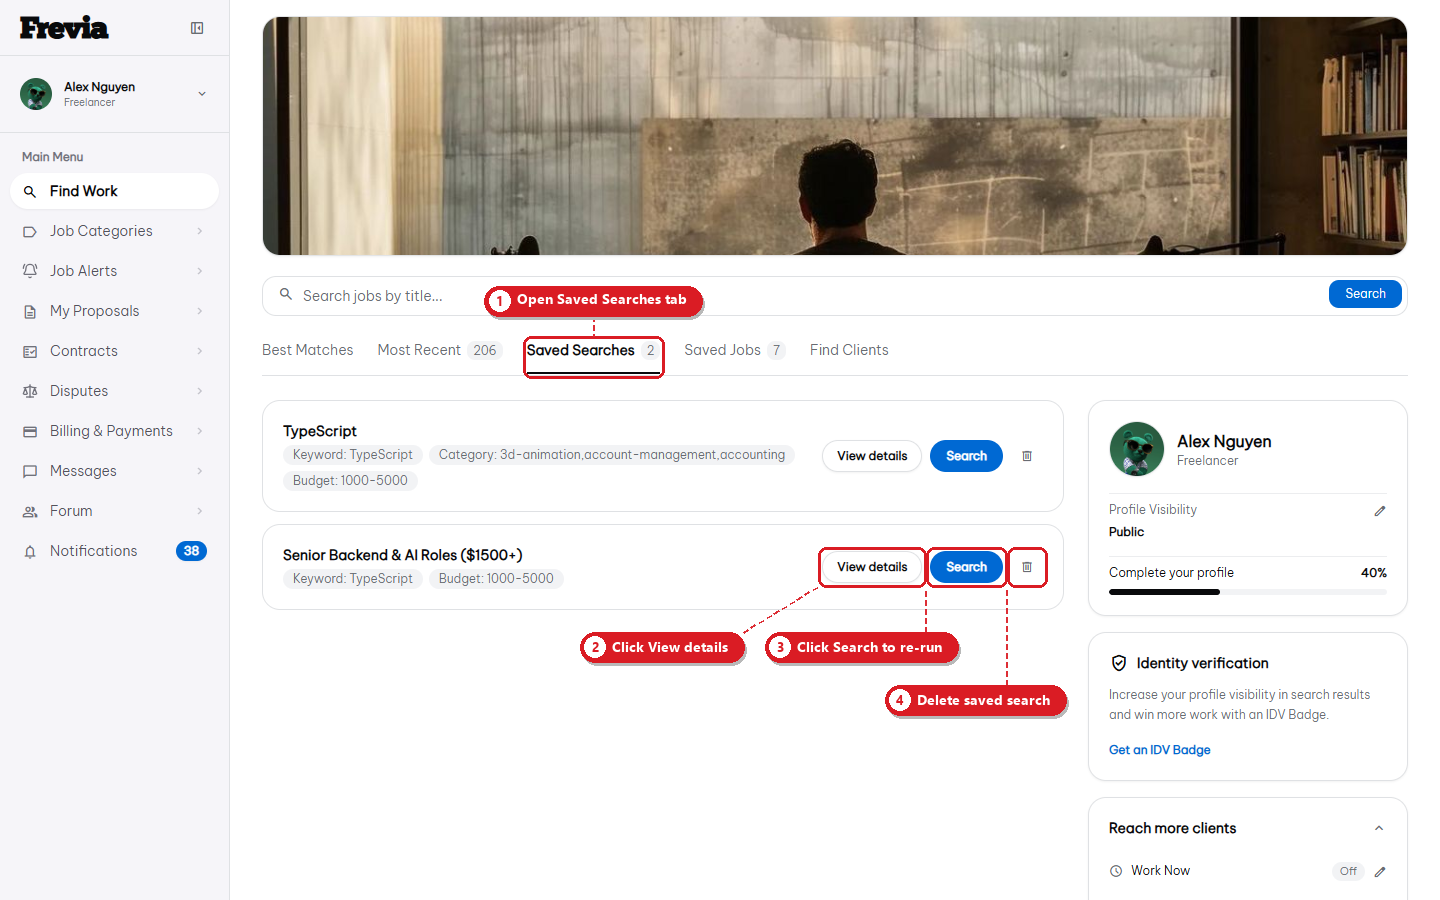
\includegraphics[width=0.90\textwidth]{images/jobs_proposals/m22_01_view_saved_searches_guide.png}
  \caption{Saved Searches tab listing saved filter presets with View details, Search, and Delete actions}
  \label{fig:m22_01_view_saved_searches}
\end{figure}
\Needspace{6\baselineskip}\paragraph{Step-by-Step User Guide:}
\begin{enumerate}[leftmargin=1.8em,itemsep=3pt]
  \item \rbadge{1} \textbf{Open Saved Searches Tab:} Click \textbf{Saved Searches} in the Find Work tab bar to inspect all saved query presets.
  \item \rbadge{2} \textbf{Inspect Filter Details:} Click \textbf{View details} on any preset card to open the filter breakdown modal.
  \item \rbadge{3} \textbf{Re-run Search Immediately:} Click the blue \textbf{Search} button to execute that saved keyword, budget, and category combination directly in the job search catalog.
  \item \rbadge{4} \textbf{Delete Obsolete Presets:} Click the trash icon on the right side of a card to remove an unused saved search.
\end{enumerate}
\Needspace{6\baselineskip}\paragraph{After You Submit (Result \& Troubleshooting):}
\begin{itemize}[leftmargin=1.5em,itemsep=2pt]
  \item \textbf{What Happens Next:} Your saved search presets display their custom names alongside keyword, budget, and category summary pills.
  \item \textbf{Troubleshooting \& Common Messages:} If no presets are saved yet, navigate to \texttt{/freelancer/search/jobs} to configure filters and save your first search.
\end{itemize}

% -----------------------------------------------------------------------------
\newpage
\subsubsection{M22.02 -- View Saved Search Details (UC-24.02)}

\begin{itemize}[leftmargin=1.5em,itemsep=2pt]
  \item \textbf{Screen Name \& Route Path:} Saved Search Detail Modal -- \texttt{/freelancer/\allowbreak{}find-work/\allowbreak{}saved-searches}.
  \item \textbf{Target Actor:} Freelancer.
  \item \Needspace{6\baselineskip}\textbf{Before You Begin:} Click \textbf{View details} on any saved search item in the Saved Searches list.
\end{itemize}
\begin{figure}[H]\centering
  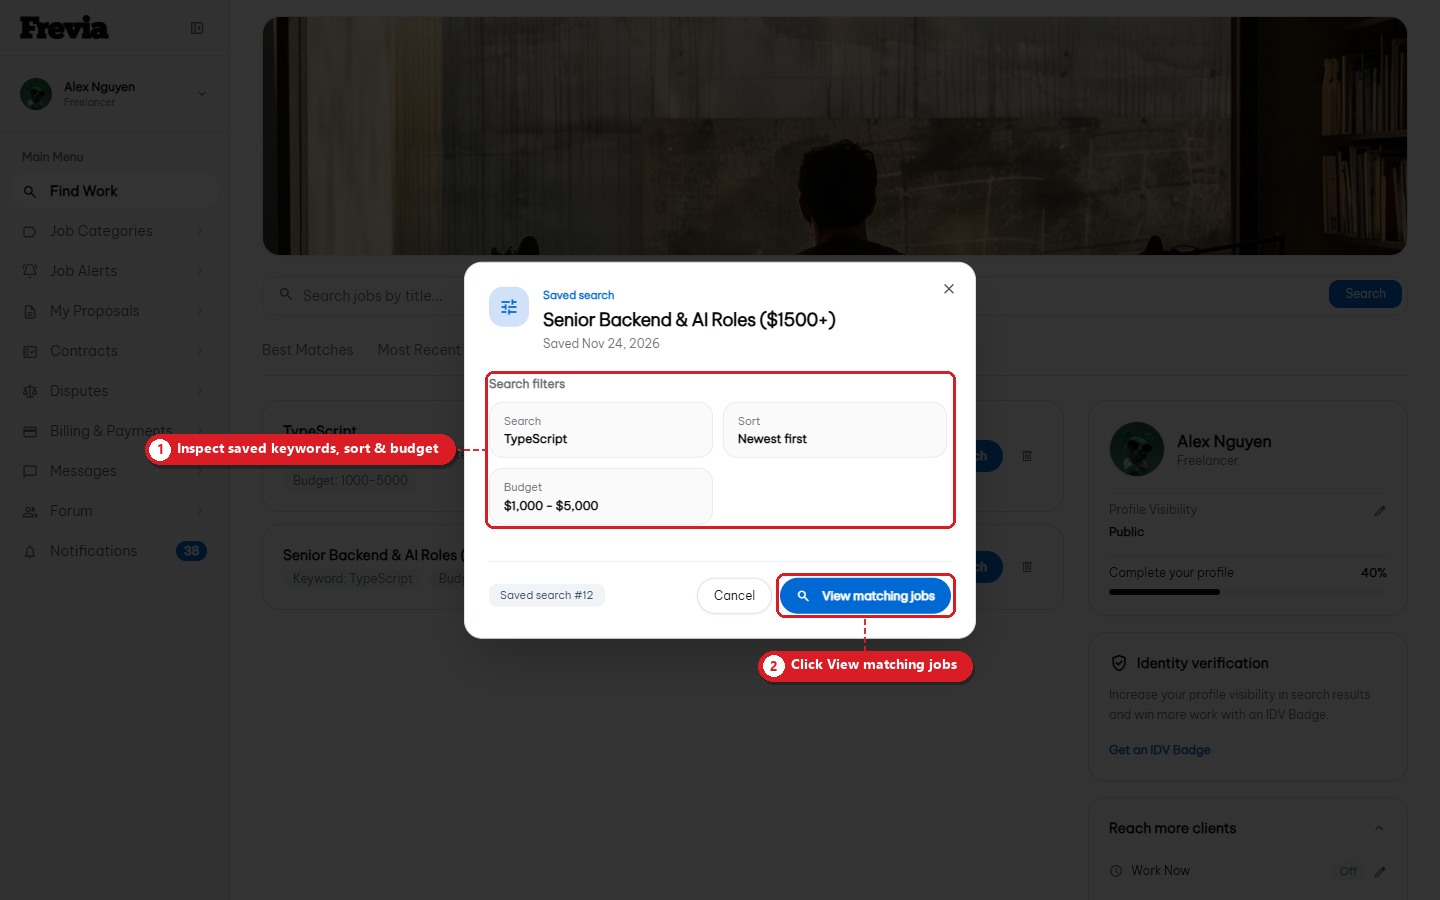
\includegraphics[width=0.90\textwidth]{images/jobs_proposals/m22_02_view_saved_search_detail_guide.png}
  \caption{Saved Search detail modal showing stored keywords, sort order, budget bounds, and quick launch}
  \label{fig:m22_02_view_saved_search_detail}
\end{figure}
\Needspace{6\baselineskip}\paragraph{Step-by-Step User Guide:}
\begin{enumerate}[leftmargin=1.8em,itemsep=3pt]
  \item \rbadge{1} \textbf{Inspect Saved Criteria:} Review the stored search keyword, sort order (\textit{Newest first}), budget range, and creation date inside the \textbf{Search filters} panel.
  \item \rbadge{2} \textbf{Launch Matching Jobs:} Click the blue \textbf{View matching jobs} button to jump straight to the filtered job search results (or \textbf{Cancel} to close).
\end{enumerate}
\Needspace{6\baselineskip}\paragraph{After You Submit (Result \& Troubleshooting):}
\begin{itemize}[leftmargin=1.5em,itemsep=2pt]
  \item \textbf{What Happens Next:} The search catalog opens pre-populated with every parameter stored in the JSON \texttt{searchParams} object.
  \item \textbf{Troubleshooting \& Common Messages:} Attempting to open a saved search owned by another user or already deleted returns HTTP 404 \textit{SavedSearchNotFound}.
\end{itemize}

% -----------------------------------------------------------------------------
\newpage
\subsubsection{M22.03 -- Create Saved Search (UC-24.03)}

\begin{itemize}[leftmargin=1.5em,itemsep=2pt]
  \item \textbf{Screen Name \& Route Path:} Save Search Dialog -- \texttt{/freelancer/\allowbreak{}search/\allowbreak{}jobs}.
  \item \textbf{Target Actor:} Freelancer.
  \item \Needspace{6\baselineskip}\textbf{Before You Begin:} Enter at least one search keyword or sidebar filter on \texttt{/freelancer/search/jobs} and click \textbf{Save search}.
\end{itemize}
\begin{figure}[H]\centering
  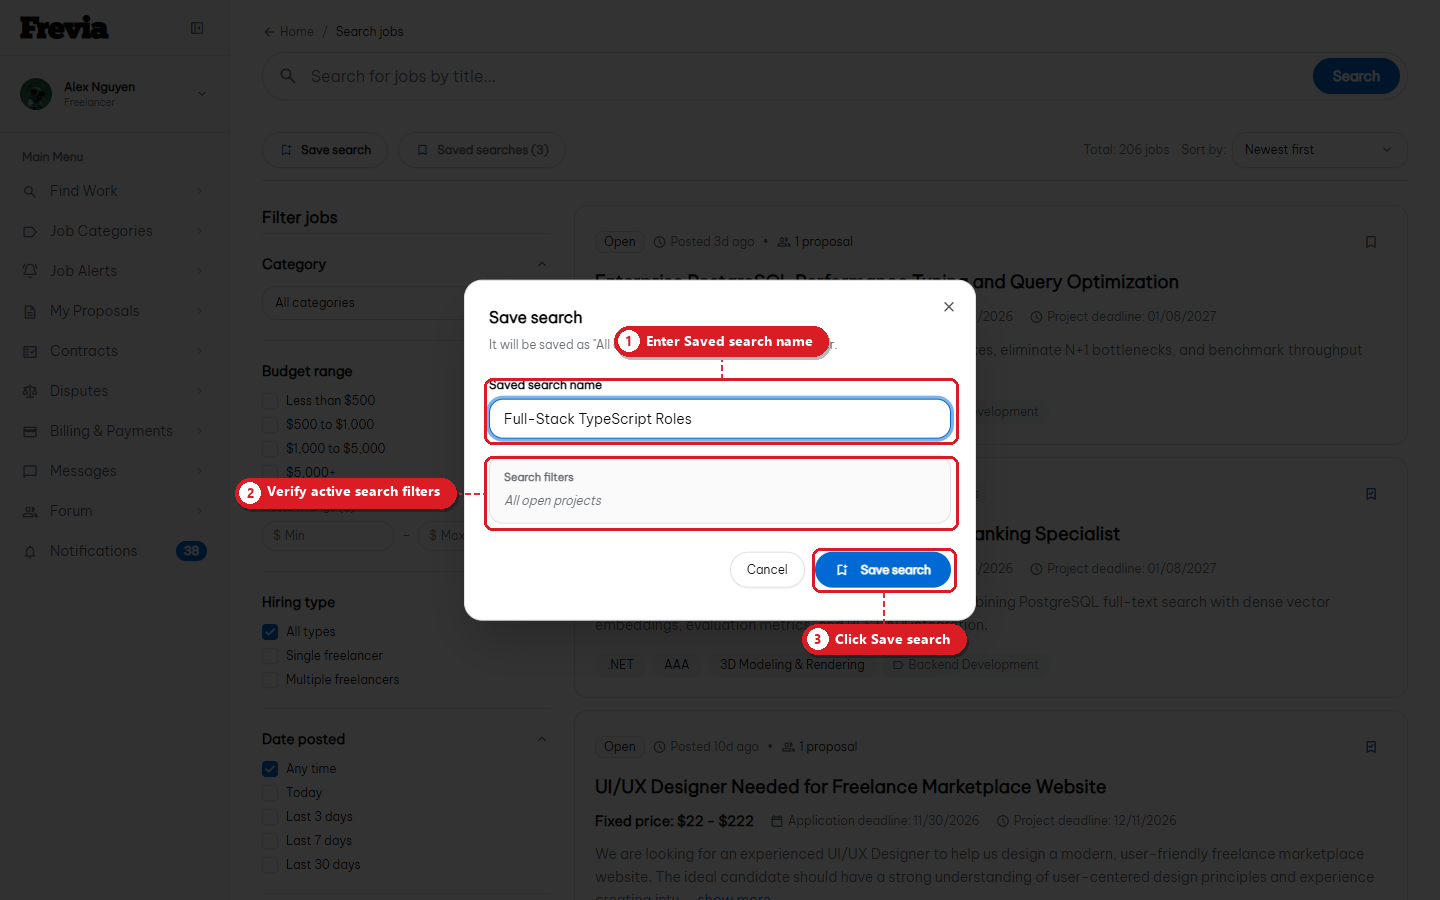
\includegraphics[width=0.90\textwidth]{images/jobs_proposals/m22_03_create_saved_search_guide.png}
  \caption{Save Search modal for naming and storing the current job filter combination}
  \label{fig:m22_03_create_saved_search}
\end{figure}
\Needspace{6\baselineskip}\paragraph{Step-by-Step User Guide:}
\begin{enumerate}[leftmargin=1.8em,itemsep=3pt]
  \item \rbadge{1} \textbf{Enter Saved Search Name:} Type a descriptive label (e.g., \textit{Full-Stack Web Roles (\$500-\$5000)}) into the \textit{Saved search name} field.
  \item \rbadge{2} \textbf{Verify Active Filters:} Confirm the summarized search keywords, category, and budget parameters listed in the \textbf{Search filters} preview card.
  \item \rbadge{3} \textbf{Click Save Search:} Click the blue \textbf{Save search} button to persist the preset to your account.
\end{enumerate}
\Needspace{6\baselineskip}\paragraph{After You Submit (Result \& Troubleshooting):}
\begin{itemize}[leftmargin=1.5em,itemsep=2pt]
  \item \textbf{What Happens Next:} The saved search is created immediately and becomes selectable under \textbf{Find Work} $\rightarrow$ \textbf{Saved Searches}.
  \item \textbf{Troubleshooting \& Common Messages:} Empty names or exceeding the per-user saved search limit trigger inline validation or HTTP 400 limit alerts.
\end{itemize}

% -----------------------------------------------------------------------------
\newpage
\subsubsection{M22.04 -- Delete Saved Search (UC-24.04)}

\begin{itemize}[leftmargin=1.5em,itemsep=2pt]
  \item \textbf{Screen Name \& Route Path:} Delete Saved Search Confirmation Dialog -- \texttt{/freelancer/\allowbreak{}find-work/\allowbreak{}saved-searches}.
  \item \textbf{Target Actor:} Freelancer (Owner).
  \item \Needspace{6\baselineskip}\textbf{Before You Begin:} Open \textbf{Find Work} $\rightarrow$ \textbf{Saved Searches} and click the trash icon on the saved search card you want to remove.
\end{itemize}
\begin{figure}[H]\centering
  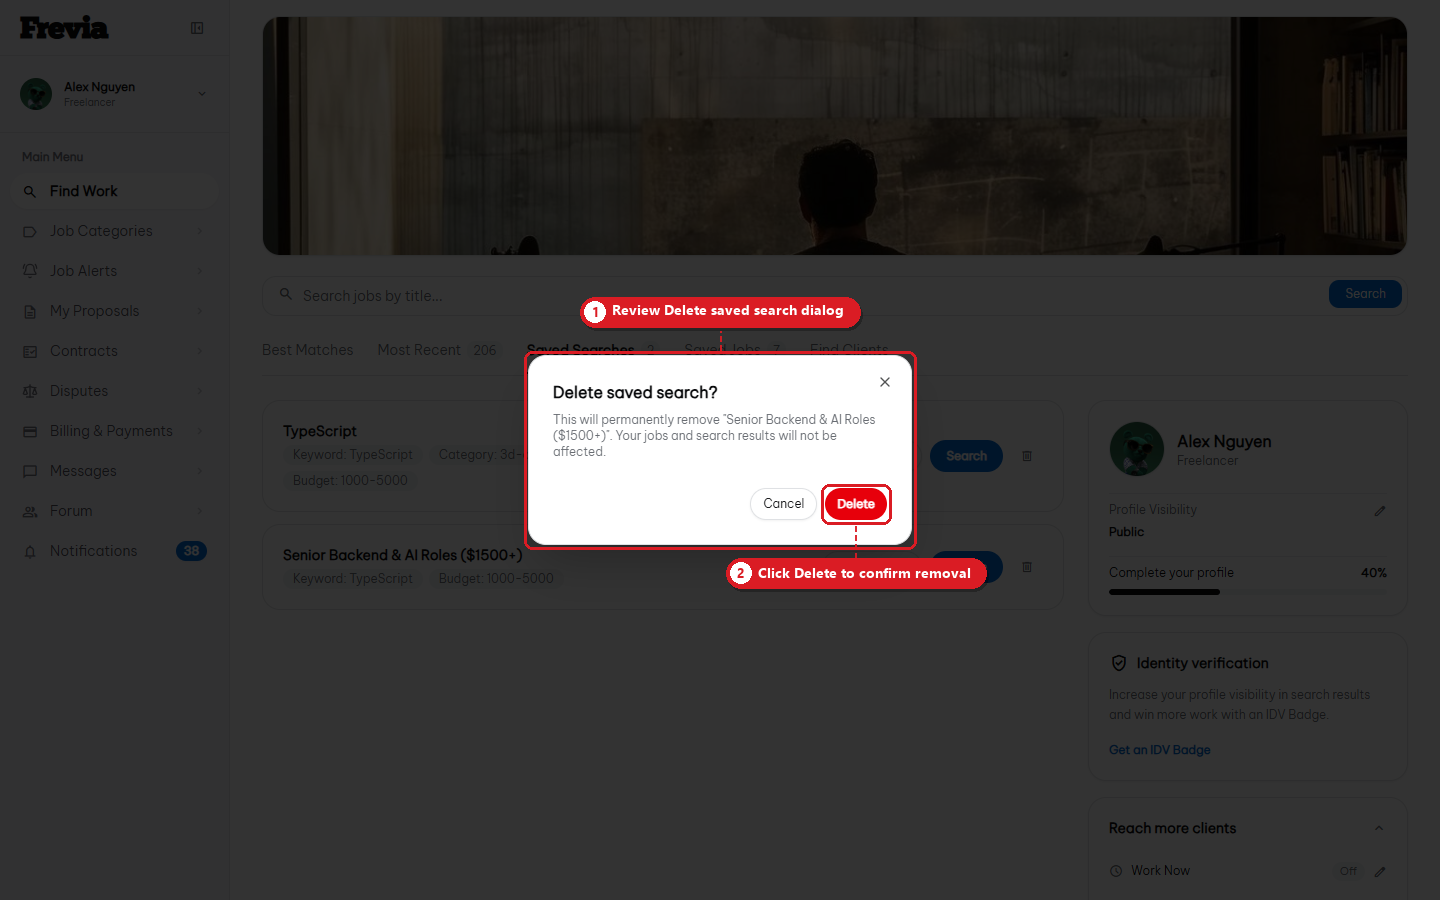
\includegraphics[width=0.90\textwidth]{images/jobs_proposals/m22_04_delete_saved_search_guide.png}
  \caption{Delete saved search confirmation dialog to permanently remove a saved filter preset}
  \label{fig:m22_04_delete_saved_search}
\end{figure}
\Needspace{6\baselineskip}\paragraph{Step-by-Step User Guide:}
\begin{enumerate}[leftmargin=1.8em,itemsep=3pt]
  \item \rbadge{1} \textbf{Review Delete Confirmation Dialog:} Inspect the \textbf{Delete saved search?} prompt naming the preset to be permanently removed while keeping your jobs and search results unaffected.
  \item \rbadge{2} \textbf{Click Delete to Confirm:} Click the red \textbf{Delete} button to remove the preset (or \textbf{Cancel} to keep it).
\end{enumerate}
\Needspace{6\baselineskip}\paragraph{After You Submit (Result \& Troubleshooting):}
\begin{itemize}[leftmargin=1.5em,itemsep=2pt]
  \item \textbf{What Happens Next:} The saved search record is permanently deleted from PostgreSQL, a green \textit{Saved search deleted} toast appears, and the Saved Searches tab counter decrements automatically.
  \item \textbf{Troubleshooting \& Common Messages:} Deleting a non-existent or non-owned ID returns HTTP 404 \textit{SavedSearchNotFound}.
\end{itemize}

% -----------------------------------------------------------------------------
\newpage
\subsubsection{M23.01 -- View Job Alerts List (UC-25.01)}

\begin{itemize}[leftmargin=1.5em,itemsep=2pt]
  \item \textbf{Screen Name \& Route Path:} Job Alerts Management -- \texttt{/freelancer/\allowbreak{}job-alerts}.
  \item \textbf{Target Actor:} Freelancer.
  \item \Needspace{6\baselineskip}\textbf{Before You Begin:} Sign in to the Freelancer workspace.
\end{itemize}
\begin{figure}[H]\centering
  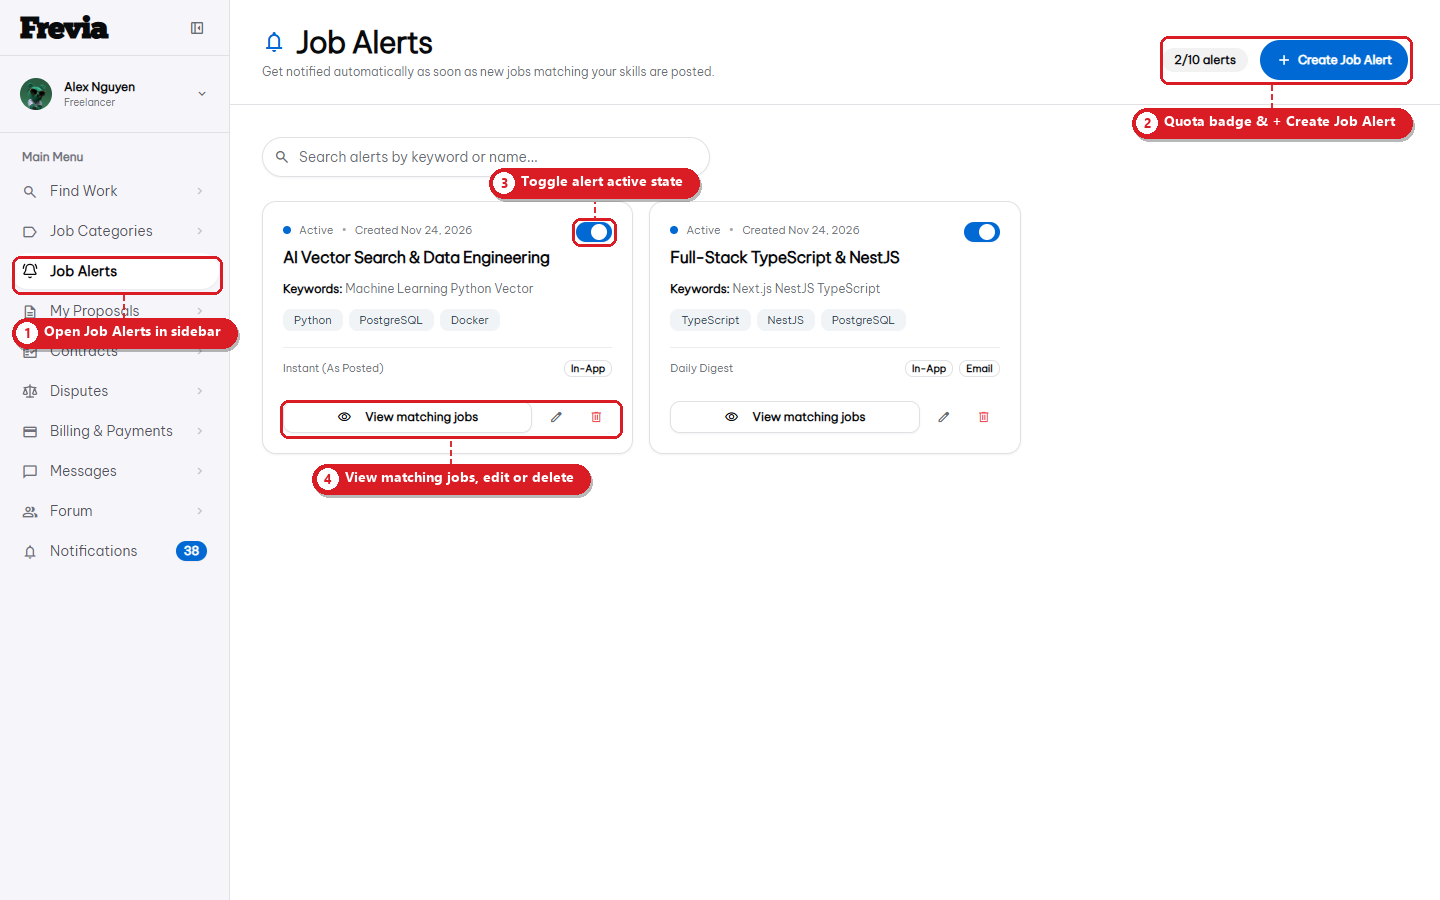
\includegraphics[width=0.90\textwidth]{images/jobs_proposals/m23_01_view_job_alerts_guide.png}
  \caption{Job Alerts management grid showing quota pill, active toggle switches, and card actions}
  \label{fig:m23_01_view_job_alerts}
\end{figure}
\Needspace{6\baselineskip}\paragraph{Step-by-Step User Guide:}
\begin{enumerate}[leftmargin=1.8em,itemsep=3pt]
  \item \rbadge{1} \textbf{Open Job Alerts:} Click \textbf{Job Alerts} in the left navigation sidebar.
  \item \rbadge{2} \textbf{Check Quota \& Create Alert:} Review your current usage pill (up to \textbf{10 alerts} per Freelancer) and click \textbf{+ Create Job Alert} to add a new rule.
  \item \rbadge{3} \textbf{Toggle Active Status:} Use the blue switch at the top-right of any alert card to pause or resume notifications without deleting the alert.
  \item \rbadge{4} \textbf{Inspect Matches, Edit or Delete:} Click \textbf{View matching jobs} to preview matching open postings, or use the pencil and trash icons to modify or delete the alert.
\end{enumerate}
\Needspace{6\baselineskip}\paragraph{After You Submit (Result \& Troubleshooting):}
\begin{itemize}[leftmargin=1.5em,itemsep=2pt]
  \item \textbf{What Happens Next:} All configured alerts display their keywords, skill chips, delivery frequency (\textit{Instant}, \textit{Daily Digest}, \textit{Weekly}), and active channels (\textit{In-App}, \textit{Email}).
  \item \textbf{Troubleshooting \& Common Messages:} Use the top search box to filter alerts by name or keyword when managing multiple alert rules.
\end{itemize}

% -----------------------------------------------------------------------------
\newpage
\subsubsection{M23.02 -- View Job Alert Details \& Matching Jobs (UC-25.02)}

\begin{itemize}[leftmargin=1.5em,itemsep=2pt]
  \item \textbf{Screen Name \& Route Path:} Job Alert Details Modal -- \texttt{/freelancer/\allowbreak{}job-alerts}.
  \item \textbf{Target Actor:} Freelancer (Owner).
  \item \Needspace{6\baselineskip}\textbf{Before You Begin:} Click \textbf{View matching jobs} on any configured alert card in \texttt{/freelancer/job-alerts}.
\end{itemize}
\begin{figure}[H]\centering
  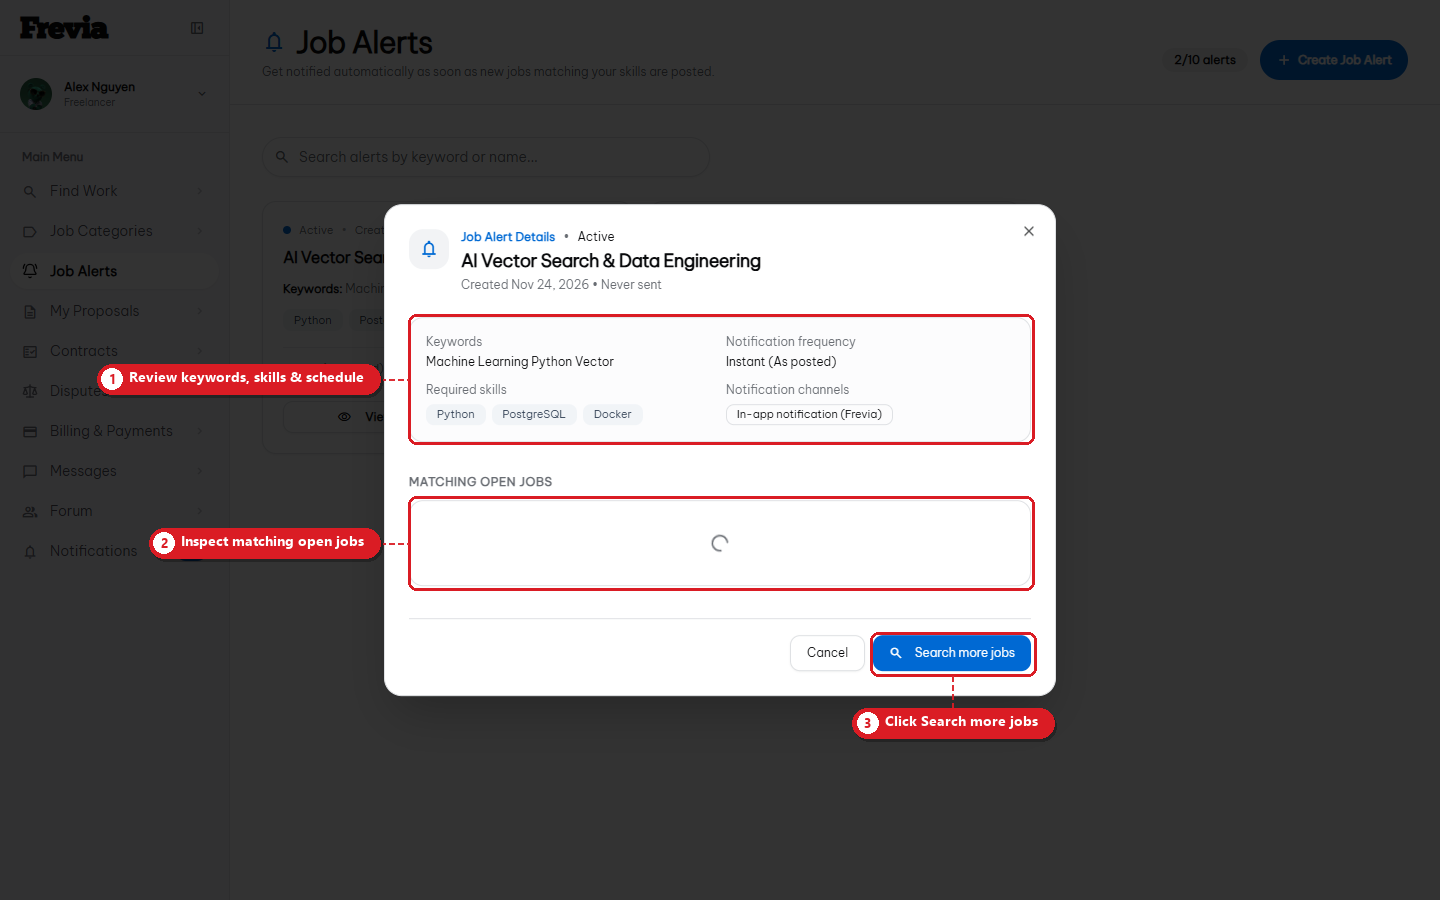
\includegraphics[width=0.90\textwidth]{images/jobs_proposals/m23_02_view_job_alert_detail_guide.png}
  \caption{Job Alert Details modal presenting alert criteria, matching open jobs preview, and full search link}
  \label{fig:m23_02_view_job_alert_detail}
\end{figure}
\Needspace{6\baselineskip}\paragraph{Step-by-Step User Guide:}
\begin{enumerate}[leftmargin=1.8em,itemsep=3pt]
  \item \rbadge{1} \textbf{Review Alert Criteria:} Inspect the alert's active state, stored \textit{Keywords}, \textit{Required skills}, \textit{Notification frequency}, and \textit{Notification channels}.
  \item \rbadge{2} \textbf{Inspect Matching Open Jobs:} Review the live preview of currently \texttt{OPEN} jobs matching your alert criteria directly inside the \textbf{MATCHING OPEN JOBS} panel.
  \item \rbadge{3} \textbf{Explore Full Results:} Click the blue \textbf{Search more jobs} button to open the full Find Work search view with those criteria pre-applied.
\end{enumerate}
\Needspace{6\baselineskip}\paragraph{After You Submit (Result \& Troubleshooting):}
\begin{itemize}[leftmargin=1.5em,itemsep=2pt]
  \item \textbf{What Happens Next:} Matching open jobs from non-banned Clients load live without altering your alert configuration.
  \item \textbf{Troubleshooting \& Common Messages:} If zero jobs currently match, broaden your keywords or remove overly restrictive skills via the Edit modal.
\end{itemize}

% -----------------------------------------------------------------------------
\newpage
\subsubsection{M23.03 -- Create Job Alert (UC-25.03)}

\begin{itemize}[leftmargin=1.5em,itemsep=2pt]
  \item \textbf{Screen Name \& Route Path:} Create Job Alert Dialog -- \texttt{/freelancer/\allowbreak{}job-alerts}.
  \item \textbf{Target Actor:} Freelancer.
  \item \Needspace{6\baselineskip}\textbf{Before You Begin:} Ensure you have fewer than 10 existing job alerts and click \textbf{+ Create Job Alert}.
\end{itemize}
\begin{figure}[H]\centering
  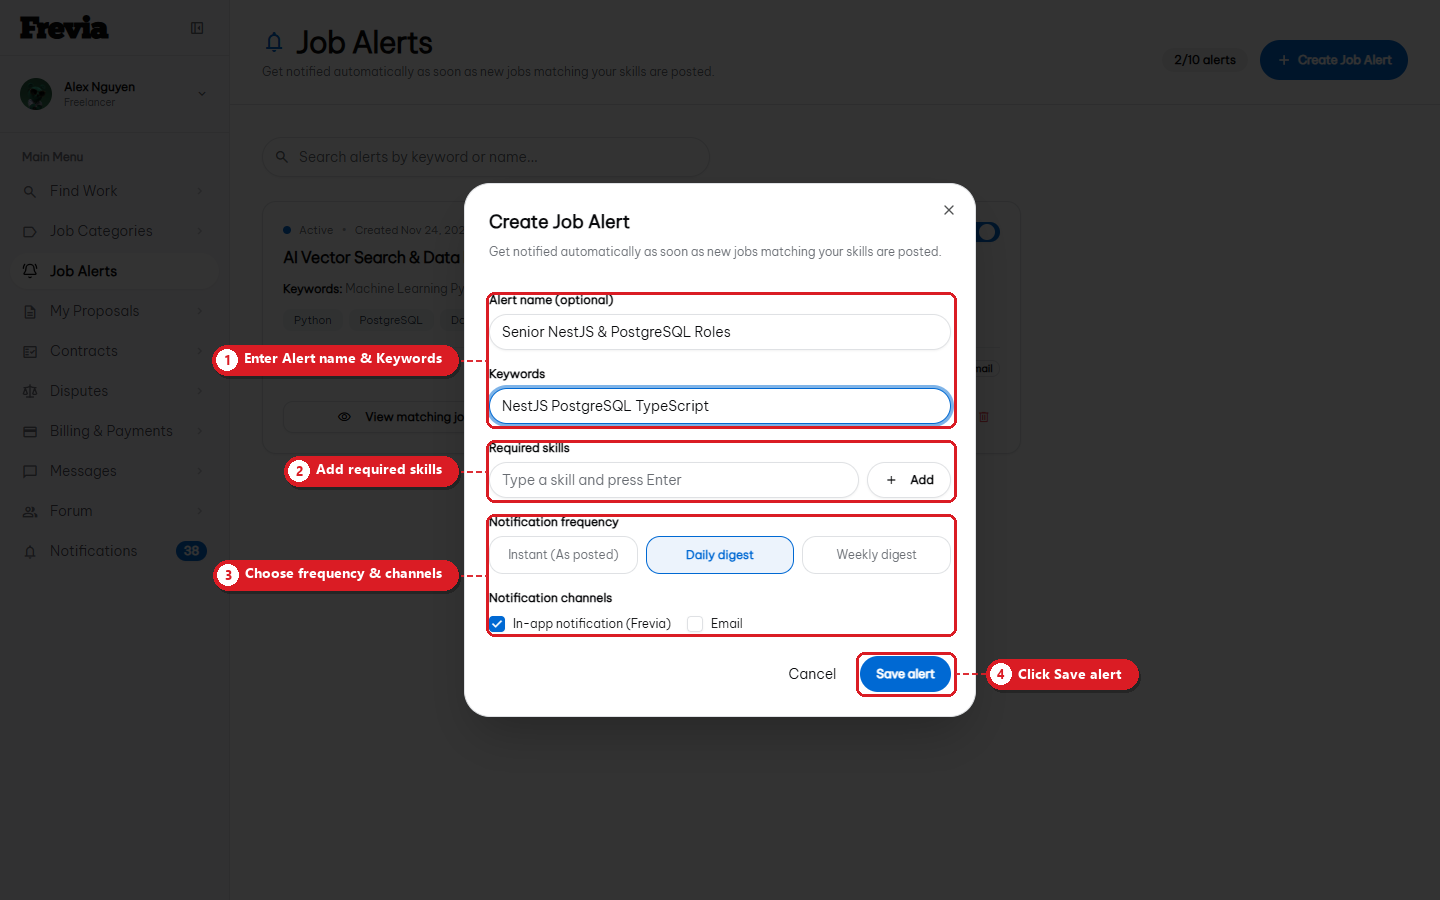
\includegraphics[width=0.90\textwidth]{images/jobs_proposals/m23_03_create_job_alert_guide.png}
  \caption{Create Job Alert modal for defining keywords, skills, notification frequency, and delivery channels}
  \label{fig:m23_03_create_job_alert}
\end{figure}
\Needspace{6\baselineskip}\paragraph{Step-by-Step User Guide:}
\begin{enumerate}[leftmargin=1.8em,itemsep=3pt]
  \item \rbadge{1} \textbf{Enter Alert Name \& Keywords:} Optionally name the alert and enter search \textit{Keywords} (e.g., \textit{NestJS PostgreSQL TypeScript}).
  \item \rbadge{2} \textbf{Add Required Skills:} Type a skill tag and press Enter (or click \textbf{+ Add}) to include skill-based matching criteria.
  \item \rbadge{3} \textbf{Choose Frequency \& Channels:} Select \textbf{Instant (As posted)}, \textbf{Daily digest}, or \textbf{Weekly digest}, and check at least one channel (\textbf{In-app notification} and/or \textbf{Email}).
  \item \rbadge{4} \textbf{Click Save Alert:} Click the blue \textbf{Save alert} button to activate automated job matching.
\end{enumerate}
\Needspace{6\baselineskip}\paragraph{After You Submit (Result \& Troubleshooting):}
\begin{itemize}[leftmargin=1.5em,itemsep=2pt]
  \item \textbf{What Happens Next:} The new alert appears immediately on \texttt{/freelancer/job-alerts} in \textit{Active} state and increments your \texttt{X/10 alerts} counter.
  \item \textbf{Troubleshooting \& Common Messages:} At least one keyword or skill is required; duplicate criteria (identical normalized keywords and skills) or exceeding 10 alerts return HTTP 400 validation notices.
\end{itemize}

% -----------------------------------------------------------------------------
\newpage
\subsubsection{M23.04 -- Update Job Alert (UC-25.04)}

\begin{itemize}[leftmargin=1.5em,itemsep=2pt]
  \item \textbf{Screen Name \& Route Path:} Edit Job Alert Dialog -- \texttt{/freelancer/\allowbreak{}job-alerts}.
  \item \textbf{Target Actor:} Freelancer (Owner).
  \item \Needspace{6\baselineskip}\textbf{Before You Begin:} Click the pencil (Edit) icon on any existing alert card in \texttt{/freelancer/job-alerts}.
\end{itemize}
\begin{figure}[H]\centering
  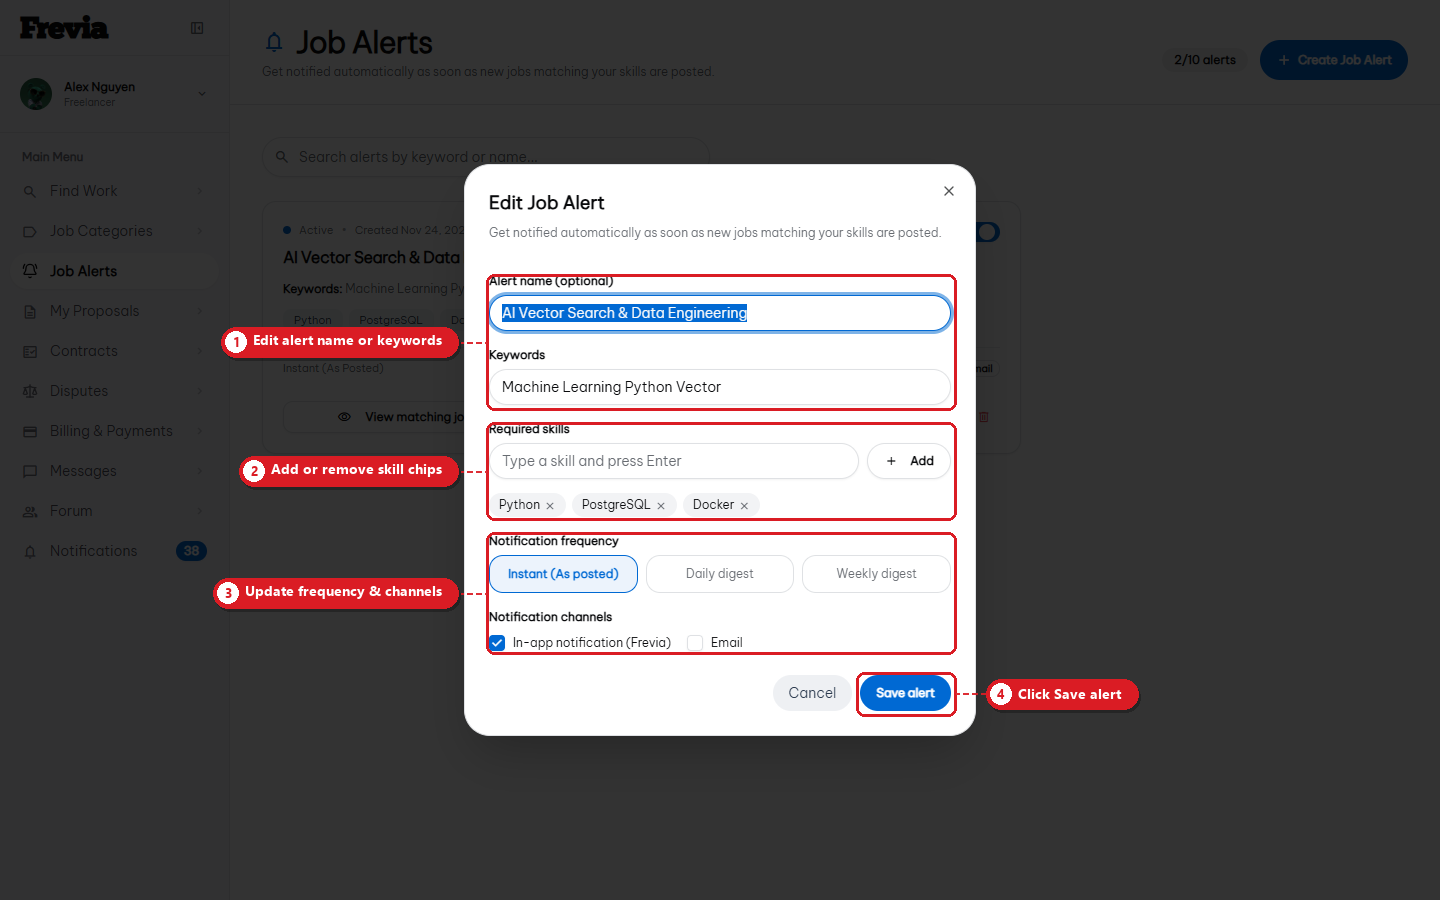
\includegraphics[width=0.90\textwidth]{images/jobs_proposals/m23_04_update_job_alert_guide.png}
  \caption{Edit Job Alert modal pre-populated with current alert settings and skill chips}
  \label{fig:m23_04_update_job_alert}
\end{figure}
\Needspace{6\baselineskip}\paragraph{Step-by-Step User Guide:}
\begin{enumerate}[leftmargin=1.8em,itemsep=3pt]
  \item \rbadge{1} \textbf{Edit Name or Keywords:} Modify the \textit{Alert name} or \textit{Keywords} input field.
  \item \rbadge{2} \textbf{Update Skill Chips:} Remove existing skill tags via the \texttt{x} icon or add new skills using \textbf{+ Add}.
  \item \rbadge{3} \textbf{Change Frequency or Channels:} Switch delivery cadence or toggle \textbf{In-app notification} and \textbf{Email} checkboxes.
  \item \rbadge{4} \textbf{Click Save Alert:} Click the blue \textbf{Save alert} button to persist your updated criteria (or \textbf{Cancel} to discard).
\end{enumerate}
\Needspace{6\baselineskip}\paragraph{After You Submit (Result \& Troubleshooting):}
\begin{itemize}[leftmargin=1.5em,itemsep=2pt]
  \item \textbf{What Happens Next:} The alert card updates immediately and subsequent job matches use the revised configuration.
  \item \textbf{Troubleshooting \& Common Messages:} Updating criteria so they duplicate another existing alert returns HTTP 400 \textit{DuplicateJobAlert}.
\end{itemize}

% -----------------------------------------------------------------------------
\newpage
\subsubsection{M23.05 -- Delete Job Alert (UC-25.05)}

\begin{itemize}[leftmargin=1.5em,itemsep=2pt]
  \item \textbf{Screen Name \& Route Path:} Delete Job Alert Confirmation Dialog -- \texttt{/freelancer/\allowbreak{}job-alerts}.
  \item \textbf{Target Actor:} Freelancer (Owner).
  \item \Needspace{6\baselineskip}\textbf{Before You Begin:} Click the red trash icon on the alert card you wish to remove.
\end{itemize}
\begin{figure}[H]\centering
  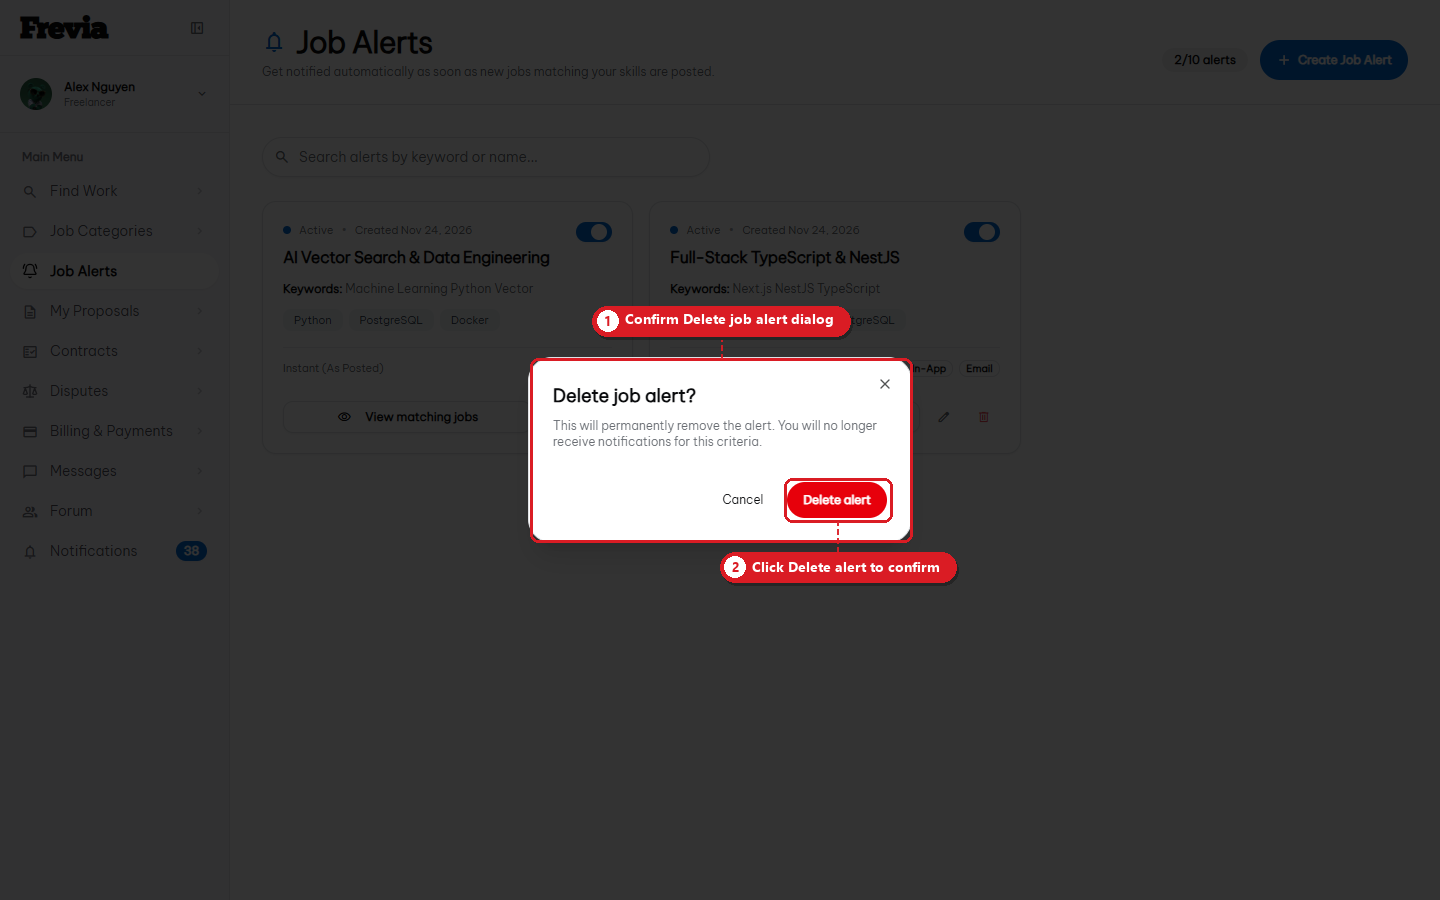
\includegraphics[width=0.90\textwidth]{images/jobs_proposals/m23_05_delete_job_alert_guide.png}
  \caption{Delete job alert confirmation dialog to permanently remove an alert rule}
  \label{fig:m23_05_delete_job_alert}
\end{figure}
\Needspace{6\baselineskip}\paragraph{Step-by-Step User Guide:}
\begin{enumerate}[leftmargin=1.8em,itemsep=3pt]
  \item \rbadge{1} \textbf{Review Removal Warning:} Confirm you want to permanently stop receiving notifications for this alert's criteria.
  \item \rbadge{2} \textbf{Click Delete Alert:} Click the red \textbf{Delete alert} button (or \textbf{Cancel} to retain the alert).
\end{enumerate}
\Needspace{6\baselineskip}\paragraph{After You Submit (Result \& Troubleshooting):}
\begin{itemize}[leftmargin=1.5em,itemsep=2pt]
  \item \textbf{What Happens Next:} The alert is permanently removed and frees up 1 slot in your 10-alert quota.
  \item \textbf{Troubleshooting \& Common Messages:} Attempting to delete an alert already removed in another session returns HTTP 404 \textit{JobAlertNotFound}.
\end{itemize}

% -----------------------------------------------------------------------------
\newpage
\subsubsection{M46.07 -- View Job Categories List (UC-50.01)}

\begin{itemize}[leftmargin=1.5em,itemsep=2pt]
  \item \textbf{Screen Name \& Route Path:} Explore Job Categories -- \texttt{/freelancer/\allowbreak{}categories}.
  \item \textbf{Target Actor:} Freelancer, Guest.
  \item \Needspace{6\baselineskip}\textbf{Before You Begin:} Open \textbf{Job Categories} from the Freelancer sidebar navigation.
\end{itemize}
\begin{figure}[H]\centering
  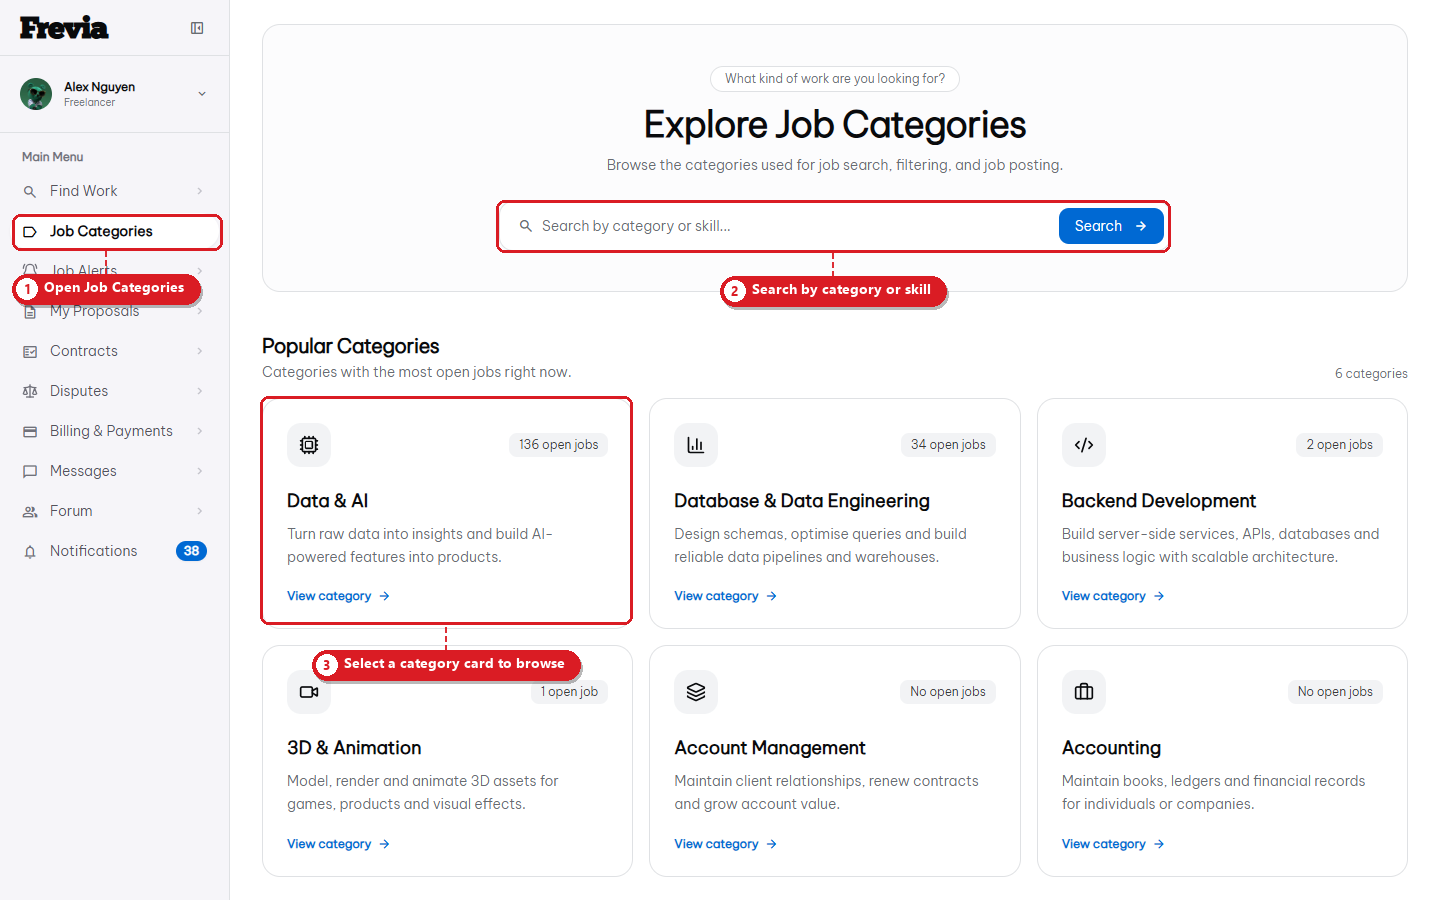
\includegraphics[width=0.90\textwidth]{images/jobs_proposals/m46_07_view_job_categories_guide.png}
  \caption{Explore Job Categories directory with live search and Popular Categories open-job counts}
  \label{fig:m46_07_view_job_categories}
\end{figure}
\Needspace{6\baselineskip}\paragraph{Step-by-Step User Guide:}
\begin{enumerate}[leftmargin=1.8em,itemsep=3pt]
  \item \rbadge{1} \textbf{Open Job Categories:} Click \textbf{Job Categories} in the left sidebar to load the active discipline catalog.
  \item \rbadge{2} \textbf{Search Categories:} Type a discipline name or keyword (e.g., \textit{Data}, \textit{Backend}) into \textit{Search by category or skill...} and click \textbf{Search}.
  \item \rbadge{3} \textbf{Select a Category Card:} Review open-job counter pills (e.g., \textit{136 open jobs}) and click any category card or \textbf{View category} link to explore its listings.
\end{enumerate}
\Needspace{6\baselineskip}\paragraph{After You Submit (Result \& Troubleshooting):}
\begin{itemize}[leftmargin=1.5em,itemsep=2pt]
  \item \textbf{What Happens Next:} Active categories render with cached open-job counts (5-minute TTL, automatically invalidated whenever jobs are created, published, closed, or deleted).
  \item \textbf{Troubleshooting \& Common Messages:} Soft-deleted or \texttt{INACTIVE} categories are automatically excluded from this public directory.
\end{itemize}

% -----------------------------------------------------------------------------
\newpage
\subsubsection{M46.08 -- View Job Category Details (UC-50.02)}

\begin{itemize}[leftmargin=1.5em,itemsep=2pt]
  \item \textbf{Screen Name \& Route Path:} Job Category Detail -- \texttt{/freelancer/\allowbreak{}categories/\allowbreak{}[slug]}.
  \item \textbf{Target Actor:} Freelancer, Guest.
  \item \Needspace{6\baselineskip}\textbf{Before You Begin:} Click any active category card from \texttt{/freelancer/categories} (e.g., \textit{Data \& AI}).
\end{itemize}
\begin{figure}[H]\centering
  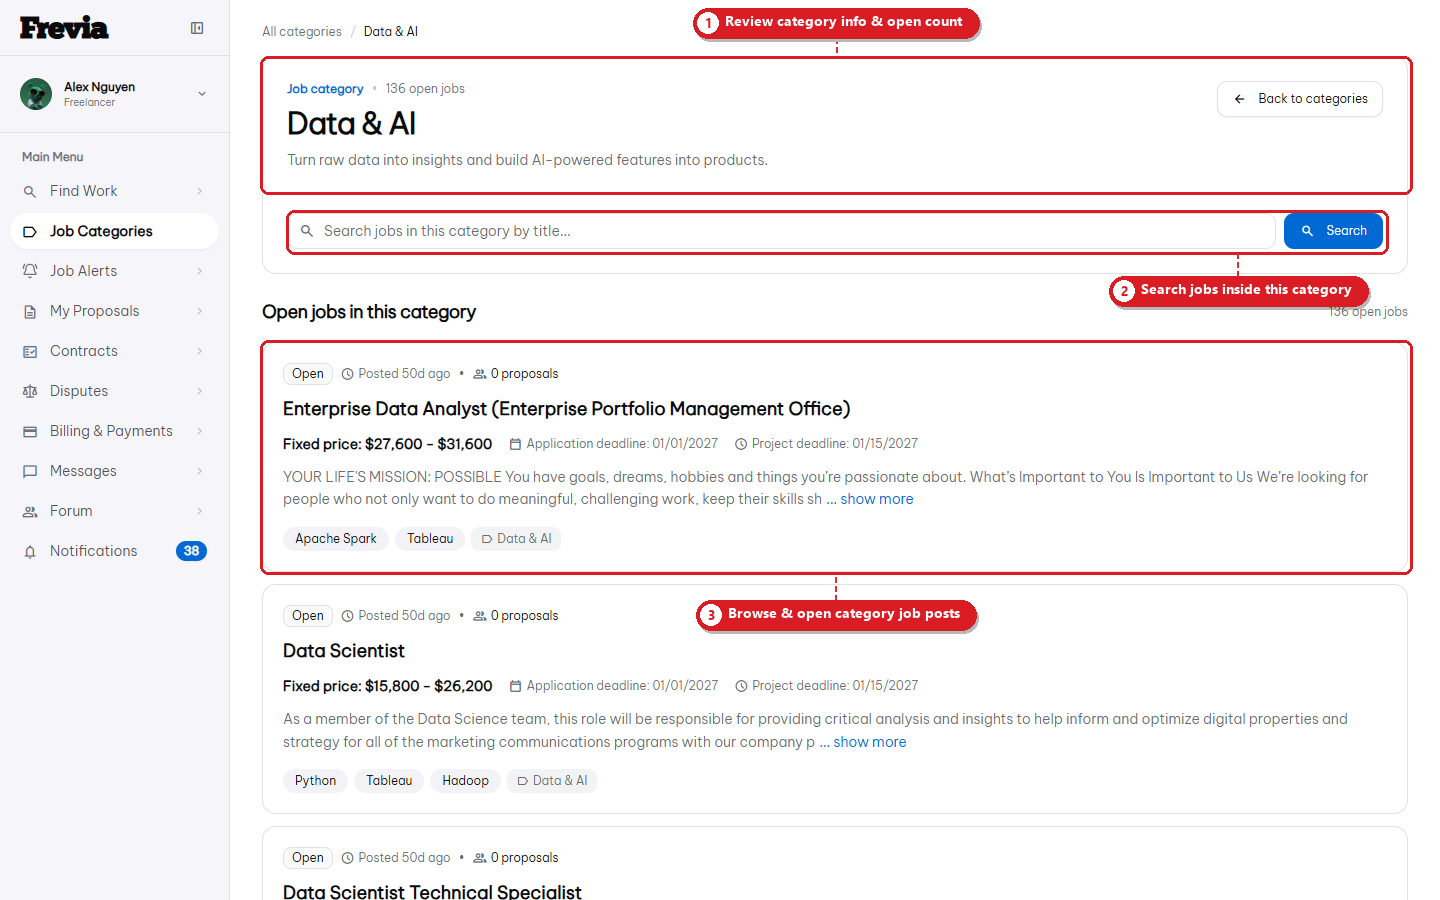
\includegraphics[width=0.90\textwidth]{images/jobs_proposals/m46_08_view_job_category_detail_guide.png}
  \caption{Job Category Detail page listing open jobs filtered to the selected discipline}
  \label{fig:m46_08_view_job_category_detail}
\end{figure}
\Needspace{6\baselineskip}\paragraph{Step-by-Step User Guide:}
\begin{enumerate}[leftmargin=1.8em,itemsep=3pt]
  \item \rbadge{1} \textbf{Inspect Category Header:} Read the category title, description, total open-job count, or click \textbf{Back to categories} to return to the directory.
  \item \rbadge{2} \textbf{Search Within Category:} Enter a job title keyword in \textit{Search jobs in this category by title...} and click \textbf{Search}.
  \item \rbadge{3} \textbf{Open Matching Job Postings:} Click any open job card below to inspect full project details, bookmark it, or submit a proposal.
\end{enumerate}
\Needspace{6\baselineskip}\paragraph{After You Submit (Result \& Troubleshooting):}
\begin{itemize}[leftmargin=1.5em,itemsep=2pt]
  \item \textbf{What Happens Next:} Paginated \texttt{OPEN} jobs assigned to the selected category render with budgets, deadlines, and skill chips.
  \item \textbf{Troubleshooting \& Common Messages:} Navigating to an invalid or inactive category slug displays an HTTP 404 \textit{JobCategoryNotFound} notice.
\end{itemize}
